\begin{chapter}{Kapitel}
 \section*{Chapter 2.1}
 
 \f{Verifikation}: \ku{check that we are building the thing right}
 \vspace*{3pt}
 
 \noindent Soll den Nachweis liefern, dass das System die Anforderungen immer erfüllt (Korrektheit der Implementierung in Bezug auf die Spezifikation).
 \vspace*{3pt}
 
 \f{Validation}: \ku{check that we are building the right thing}
 \vspace*{3pt}
 
 \noindent Entspricht eher dem kritischen Überprüfen der Spezifikation anhand eines ersten Designs auf Richtigkeit und Vollständigkeit.
 
 \f{Testen}: \ku{ist ein Mittel für beides und weit verbreitet.}
 \vspace*{3pt}
 
 \noindent Verifikation lässt sich damit nicht bewerkstelligen, allenfalls Falsifikation. 
 \vspace*{8pt}
 
 \f{Populäre Techniken der Verifikation}:
\begin{itemize}
 \item \f{Peer Reviewing}: Statische Methode der manuellen Durchsicht und Prüfung des Codes durch einen Experten. Im Mittel bringt dies 60\% der Fehler, subtile
 Fehler werden meist nicht gefunden.
 \item \f{Testen}: Dynamische Methode, häufig unterstützt durch Qualitätsmetriken (Code Coverage). 30\% bis 50\% der Gesamtkosten gehen auf das Konto von Testen, 
 bei Hardware sind oft 70\% des entwickelten Codes Testbenches.
\end{itemize}
Man kann mit Tests die Anwesenheit von Fehlern nachweisen, nicht jedoch deren Abwesenheit!
\vspace*{8pt}

\f{Formale Methoden}:
\vspace*{4pt}

\noindent Formale Methoden basieren auf formalen Sprachen zur Spezifikation von Eigenschaften wie auch zur Konstruktion des Systems. Gebräuchliche 
Verifikationstechniken mit formalen Methoden sind:
\begin{itemize}
 \item \f{Deduktive Methoden}: Hier liefert man einen mathematischen Beweis, dass die Implementierung die Spezifikation erfüllt. Meist werden Theorembeweiser 
 oder Beweisprüfer als Werkzeuge benutzt. Problem: Sehr aufwändig, das System muss die Form einer Mathematischen Theorie haben.
 \item \f{Model Checking}: Systematische und erschöpfende Überprüfung der Spezifikation auf allen erreichbaren Systemzuständen. Meist vollautomatisch durch 
 sogenannte Modellchecker. Problem: Zustandsraumexplosion
 \item \f{Modelbasierte Simulation und Test}: Exploration möglicher Verhalten mit Überprüfung der Spezifikationen
\end{itemize}

\f{Model-Checking}:
\vspace*{4pt}

\noindent Man betrachtet 
\begin{itemize}
 \item \f{Spezifikation}: formale Definition der Eigenschaften des gewünschten Systems in Form von Sätzen einer mathematischen Theorie (Aussagen einer temporalen 
 Logik)
 \item \f{Implementierung}: formale Definition der konkreten Konstruktion des Systems (als diskretes Transitionssystem)
 \item \f{Model Checking}: Ist die Implementierung ein Modell für die Theorie (gelten die Sätze für die Implementierung)
\end{itemize}
\begin{figure}[!ht]
 \centering
 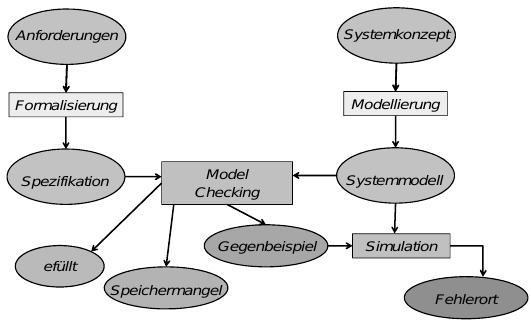
\includegraphics[scale=0.8]{pics/modelchecking}
\end{figure}

\f{Transitionssysteme}:

\f{Definition}: \ku{Ein Tupel $T=(S,(Act,)\rightarrow, St)$ heißt Transitionssystem, wobei}
\begin{itemize}
 \item $S$ \dots eine Menge von Zuständen 
 \item $\rightarrow \subseteq S\times S$ die Transitionsrelation ($\rightarrow \subseteq S\times Act \times S$)
 \item $Act$ eine Menge von Aktionen 
 \item $St \subseteq S$ eine Menge von Startzuständen ist 
\end{itemize}

\noindent Auf die Startzustände kann man auch verzichten oder auf genau einen gehen, der dann vermöge $\rightarrow$ nichtdeterministisch in $St$ verzweigt.
\vspace*{4pt}

\noindent Auch die Aktionen sind Komfort, sie machen es leichter, mehrere kooperierende Transitionssysteme zu definieren und Synchronisationsbedingungen über Aktionen zu 
formulieren. Wenn wir die Zustandsmenge endlich machen und die Aktionen als Ein/Ausgabemarkierungen auffassen, sind wir wieder bei unseren vertrauten Automaten.
\vspace*{4pt}

\noindent Bei endlicher Zustandsmenge ist auch klar, dass man die Übergangsrelation als gerichteten Graphen darstellen kann. 
\begin{figure}[!ht]
 \centering
 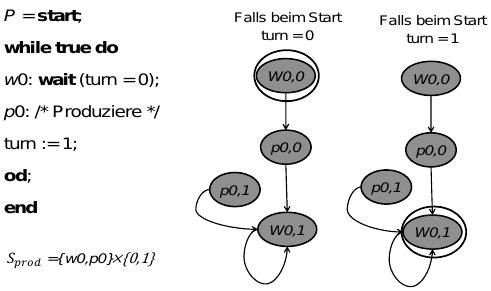
\includegraphics[scale=0.8]{pics/transitionssystem}
 \caption{Producer als Transitionssystem}
\end{figure}

\f{Kripke-Strukturen}:
\vspace*{4pt}

\noindent Praktisch stellt man Eigenschaften eines Systems durch Messung fest, d.h. Eigenschaften sind im einfachsten Falle binär, sie gelten oder gelten nicht.
\vspace*{4pt}

\noindent Alles was wir über das Verhalten eines System wissen oder erfahren können sollte sich also grundsätzlich gesehen auf endlich viele (wir können nur endlich viel 
messen) \f{atomare Aussagen} zurückführen lassen. Wir erweitern ein Transitionssystem zu einer \f{Kripke Struktur}: 

\[K = (S,(Act,)\rightarrow, St, AP, L)\]

\noindent Dabei kommen noch zwei Komponenten dazu: 
\begin{itemize}
 \item $AP$ \dots eine (endliche) Menge von atomaren Aussagen (atomic propositions)
 \item $L:S \rightarrow 2^{AP}$ \dots eine Markierung der Zustände mit den durch sie erfüllten atomaren Aussagen (labeling) 
\end{itemize}

\newpage 
\noindent Das Transitionssystem zu den Producer/Consumer-Prozessen könnte man durch folgende atomare Aussagen erweitern: \[AP=\{p,k\}\] mit $p$: es wird gerade produziert 
\\ und $k$: es wird gerade konsumiert
\vspace*{5pt}

\f{Linear-Zeit vs. Baum-Zeit}:
\vspace*{5pt}

\noindent Formal werden wir zu verifizierende Eigenschaften unserer Systeme in \f{temporaler Logik} ausdrücken. 
\vspace*{4pt}

\noindent Die \f{Linear-Zeit Logik (linear time logic, LTL)} erlaubt Aussagen über Labelings aller (unendlichen) Berechnungsfolgen der Kripke-Struktur. 
LTL-Aussagen gelten entweder für alle Folgen oder nicht. 
\vspace*{4pt}

\noindent Die \f{Baum-Zeit Logik (computation tree logic, CTL)} erlaubt die Formulierung von Aussagen über Berechnungsbäume, d.h. man kann Existenz und 
Allquantoren für die Pfade in den Unterbäumen nutzen.

\section*{Chapter 2.2}
\f{Linear-Time Logic} 
\vspace*{3pt}

\noindent Linear-Zeit Logik ist eine Logik, die auf Sequenzen von Belegungen mit atomaren Eigenschaften basiert. Die Zeit ist diskret und schreitet linear voran. Es gibt 
nur eine mögliche Zukunft.
\vspace*{4pt}

\noindent Sei $AP$ die Menge der atomaren Aussagen. Dann korrespondiert das Labeling $X \subseteq AP$ zu der Tatsache, dass alle Eigenschaften $x\in X$ in dem 
Zustand gelten und alle $y\in AP\setminus X$ in diesem Zustand nicht gelten.

\noindent LTL Formeln werden nun über Mengen von unendlichen Folgen von Labelings interpretiert. D.h. wir betrachten Sequenzen $\sigma \in (2^{AP})^\omega$, wofür
ein Alphabet $\Sigma, \Sigma^\omega$ die Menge aller unendlichen Folgen über $\Sigma$ sei. 

\noindent Für $\sigma \in (2^{AP})^\omega$ sei 
\begin{itemize}
 \item $\sigma(i) \subseteq AP$ das i-te Element der Folge
 \item $\sigma^i \in (2^{AP})^\omega$ die unendliche Folge $\sigma(i)\sigma(i+1)\sigma(i+2)\dots$
\end{itemize}
\vspace*{5pt}

\f{Syntax von LTL}:
\vspace*{4pt}

\noindent Sei $AP$ eine Menge von atomaren Aussagen. Dann ist die Menge der LTL Formeln über $AP$ wie folgt definiert: 
\begin{enumerate}
 \item jedes $p\in AP$ ist eine LTL Formel 
 \item sind $\Phi_1$ und $\Phi_2$ Formeln, dann auch $\neg \Phi_1$, $\Phi_1 \vee \Phi_2$, $\f{X}\Phi_1$, $\Phi_1\f{U}\Phi_2$
 \item nichts sonst ist eine LTL Formel 
\end{enumerate}

\noindent Dies ist eine sehr minimalistische Definition. \f{X} (next) und \f{U} (until) sind temporale Operatoren. 
\vspace*{4pt}

\noindent LTL Formeln werden über (unendlichen) Folgen von Teilmengen atomarer Aussagen interpretiert. Die Semantik einer LTL-Formel $\Phi$ ist die Menge aller 
Folgen $\sigma \in (2^{AP})^\omega$, die $\Phi$ erfüllen, d.h. 
\[[[\Phi]] = \{\sigma | \sigma \vDash \Phi\}\]

\f{Erfüllung einer LTL-Formel}:
\vspace*{5pt}

\noindent Sei $\sigma \in (2^{AP})^\omega$ und sei $\Phi$ eine LTL Formel. Dann gilt $\sigma \vDash \Phi$ (``$\sigma$ erfüllt $\Phi$'') nach folgender
Fallunterscheidung über die Struktur von $\Phi$:
\begin{itemize}
 \item $\sigma \vDash p$ \qquad \qquad   falls $p\in AP$ und $p\in\sigma(0)$
 \item $\sigma \vDash \neg\Phi$ \qquad  \qquad falls $\sigma \nvDash \Phi$
 \item $\sigma \vDash \Phi_1 \vee \Phi_2$ \qquad falls $\sigma \vDash \Phi_1$ oder $\sigma \vDash \Phi_2$
 \item $\sigma \vDash \f{X}\Phi$ \qquad  \qquad falls $\sigma^1 \vDash \Phi $
 \item $\sigma \vDash \Phi_1\f{U}\Phi_2$ \qquad falls $\exists i: \left(\sigma^i\vDash \Phi_2 \wedge \forall k < i:\sigma^k \vDash \Phi_1 \right)$
\end{itemize}
\vspace*{5pt}

\f{Nützliche Abkürzungen für LTL-Formeln}:
\vspace*{4pt}

\f{F} \dots finally (``irgendwann''), \f{G} \dots globally (``immer''), \f{W} \dots weak until, \f{R} \dots releases
\begin{itemize}
 \item $\Phi_1\wedge\Phi_2 \equiv \neg(\neg\Phi_1\vee\neg\Phi_2)$
 \item $\Phi_1 \rightarrow \Phi_2 \equiv \neg\Phi_1\vee\Phi_2$
 \item $true \equiv a\vee\neg a$
 \item $false \equiv \neg true$
 \item $\f{F}\Phi \equiv true\f{U}\Phi$
 \item $\f{G}\Phi \equiv \neg\f{F}\neg\Phi$
 \item $\Phi_1\f{W}\Phi_2 \equiv (\Phi_1\f{U}\Phi_2)\vee\f{G}\Phi_1$
 \item $\Phi_1\f{R}\Phi_2 \equiv \neg(\neg\Phi_1\f{U}\Phi_2)$
\end{itemize}
\vspace*{5pt}

\f{Tautologie, Unerfüllbarkeit, Äquivalenz}:
\vspace*{4pt}

\f{Tautologie}: Jede Formel $\Phi$ mit $[[\Phi]] = \left(2^{AP}\right)^\omega$ heißt Tautologie
\vspace*{4pt}

\f{Unerfüllbarkeit}: Jede Formel $\Phi$ mit $[[\Phi]] = \varnothing$ heißt unerfüllbar
\vspace*{4pt}

\f{Äquivalenz}: zwei Formeln $\Phi_1$ und $\Phi_2$ heißen äquivalent, gdw. $[[\Phi_1]] = [[\Phi_2]]$. Wir schreiben dann auch $\Phi_1 \equiv \Phi_2$
\vspace*{6pt}

\f{Idempotenz und Rekursionsgesetze}:
\vspace*{5pt}

\begin{itemize}
 \item $\f{F}\Phi \equiv \f{FF}\Phi$
 \item $\f{G}\Phi \equiv \f{GG}\Phi$
 \item $\Phi\f{U}\Psi \equiv \Phi\f{U}(\Phi\f{U}\Psi)$
 \item Rekursionsgesetze:
 \begin{itemize}
  \item $\f{F}\Phi \equiv \Phi\vee\f{XF}\Phi$
  \item $\f{G}\Phi \equiv \Phi\wedge\f{XG}\Phi$
  \item $\Phi\f{U}\Psi \equiv \Psi\vee(\Phi\wedge\f{X}(\Phi\f{U}\Psi))$
  \item $\Phi\f{W}\Psi \equiv \Psi\vee(\Phi\wedge\f{X}(\Phi\f{W}\Psi))$
 \end{itemize}
\end{itemize}
\vspace*{5pt}

\f{Sicherheitseigenschaften}:
\vspace*{4pt}

\noindent Eine Eigenschaft ist eine Sprache $L \subseteq \left(2^{AP}\right)^\omega$. Gibt es für alle $\sigma \in \left(2^{AP}\right)^\omega/L$ einen endlichen Präfix $w$,
so dass für alle $\alpha \in \left(2^{AP}\right)^\omega$ schon gilt $w\alpha \notin L$, d.h. es gibt keine zulässige Erweiterung mehr, mit der man den Präfix $w$
wieder nach $L$ bringen kann, dann nennt man $w$ einen \f{schlechten Präfix} und $L$ eine \f{Sicherheitseigenschaft}.
\vspace*{6pt}

\f{Lebendigkeitseigenschaften}:
\vspace*{4pt}

\noindent Es gilt $L \subseteq \left(2^{AP}\right)^\omega$. Gibt es für jedes $w \in \left(2^{AP}\right)^*$ ein $\alpha \in \left(2^{AP}\right)^\omega$ so dass 
wieder $w\alpha \in L$, d.h. es gibt stets eine zulässige Erweiterung, mit der man einen Präfix $w$ nach $L$ bringen kann, dann nennt man $L$ eine 
\f{Lebendigkeitseigenschaft}.
\vspace*{5pt}

\noindent Jede LTL-Eigenschaft lässt sich als Schnitt einer Sicherheitseigenschaft mit einer Lebendigkeitseigenschaft darstellen. 
\vspace*{4pt}

\f{Interpretation von LTL über Kripke-Strukturen  }
\vspace*{5pt}

\noindent Kripke Strukturen sind ja die formalen Modelle, die wir für Implementierungen von Systemen betrachten. Wenn wir nun wissen wollen, ob ein System in LTL 
formulierte Eigenschaften erfüllt, müssen wir nachprüfen, ob die Eigenschaft über den Menge aller (unendlichen) Ausführungsfolgen der Kripke Struktur gilt. 
\vspace*{4pt}

\noindent Sei $K = (S,\rightarrow, St, AP,L)$ eine Kripke-Struktur. 
\vspace*{4pt}

\noindent Eine Folge $\rho \in S^\omega$ mit $\rho(1)\in St$ und $\forall i:\rho(i)\rightarrow \rho(i+1)$ heißt Ausführung von $K$.
\vspace*{4pt}

\noindent Für eine Ausführung $\rho$ betrachten wir nun  $L(\rho) \in \left(2^{AP}\right)^\omega$ mit $\forall i: L(\rho)(i):=L(\rho(i))$, d.h. die 
Labelingfolge zur Ausführung $\rho$. 
\vspace*{4pt}

\noindent Dann bezeichnen wir mit $[[K]]$ die Menge aller möglichen Labelingsequenzen zu Ausführungen von K. 
\vspace*{4pt}

\[[[K]] = \{L(\rho)|\rho \text{ ist Ausführung von } K \}\]

\f{Das LTL-Model-Checking Problem}
\vspace*{4pt}

\noindent Das Problem ist es, zu entscheiden, ob eine Kripke Struktur, die wir aus der Implementierung abgeleitet haben, ein Modell für die Spezifikation ist. 
\vspace*{4pt}

\noindent Gegeben sei eine Kripke-Struktur $K=(S,\rightarrow, St,AP,L)$ und eine LTL-Formel $\Phi$ über $AP$. Entscheide, ob $[[K]] \subseteq [[\Phi]]$.
\vspace*{4pt} 

\noindent Es muss also für jede Ausführung $\rho$ das Labeling $L(\rho)$ die Formel $\Phi$ erfüllen. Wir schreiben dann auch $K \vDash \Phi$.

\noindent Vorsicht: es kann sowohl $K \vDash \Phi$ als auch $K \nvDash \neg\Phi$ gelten!
\vspace*{6pt}

\f{Fallstrick endliche Ausführungen}:
\vspace*{4pt}

\noindent Vorsicht: LTL Formeln werden nur über den unendlichen Ausführungen interpretiert.
\vspace*{4pt}

\noindent Wenn die Kripke Struktur zum Beispiel Deadlocks enthält (Zustände ohne Nachfolger in der Transitionsrelation), dann werden alle Ausführungen, die auf 
einem solchen Zustand enden ignoriert, weil sie endliche Länge haben. Auf solchen Ausführungen wird die Formel nicht interpretiert.
\vspace*{4pt}

\noindent Das kann im Extremfall unerwartete Konsequenzen haben: Angenommen in $K$ führt jeder Weg in einen Deadlock. Dann ist $[[K]] = \varnothing$. Damit 
erfüllt $K$ aber jede Formel!
\vspace*{6pt}

\f{LTL-Model-Checking}
\vspace*{4pt}

\noindent Wir wollen nun anschauen, wie man (im Prinzip, schnelle Heuristiken sind nach wie vor Gegenstand der aktuellen Forschung) Model Checking für LTL Formeln 
algorithmisch entscheidet:

\noindent Gegeben sei eine Kripke-Struktur $K=(S,\rightarrow, St,AP,L)$ und eine LTL-Formel $\Phi$ über $AP$. Entscheide, ob $[[K]] \subseteq [[\Phi]]$.

\noindent Im Prinzip gibt es zwei Möglichkeiten: 
\begin{enumerate}
 \item Konstruiere eine LTL-Formel $\Psi$ mit $[[K]] = [[\Psi]]$ und zeige $\Psi \rightarrow \Phi$. Dies ist sehr aufwändig.
 \item Die Menge der Ausführungen von $K$ lässt sich leicht als Sprache eines Büchi Automaten $BA(K)$ d.h. $[[K]] = L(BA(K))$ auffassen. Konstruiere einen weiteren 
 Büchi Automaten $BA(\neg \Phi)$ der die Sprache $[[\neg\Phi]]$ akzeptiert und entscheide \[L(BA(K)) \cap L(BA(\neg\Phi)) = \varnothing\]
\end{enumerate}

\f{Büchi-Automaten}
\vspace*{4pt}

\noindent Büchi-Automaten sind im Prinzip endliche Automaten mit einem anderen Akzeptanzkriterium. Ein Tupel $B=(S,S_0,A,\Delta,F)$ heißt \f{Büchi-Automat}, 
wobei
\begin{itemize}
 \item $S$ \dots eine endliche Menge von Zuständen 
 \item $S_0 \subseteq S$ eine Menge von Startzuständen 
 \item $\Delta \subseteq S\times A \times S$ die Übergangsrelation
 \item $A$ ein endliches Alphabet
 \item $F \subseteq S$ eine Menge von Endzuständen (Akzeptanzzuständen) ist.
\end{itemize}
Man kann Büchi Automaten ebenso durch Diagramme darstellen, wie man das von endlichen Automaten kennt lediglich die Sprache ist anders definiert:

\noindent Sei $B=(S,S_0,A,\Delta,F)$ ein Büchi-Automat. 

\noindent Für ein unendliches Wort $\sigma \in A^\omega$ ist $s(1)\sigma(1)s(2)\sigma(2)\dots s(i)\sigma(i)\dots$ ein Lauf in $B$ mit Beschriftung $\sigma$ 
genau dann wenn
\begin{itemize}
 \item $s(1) \in S_0$ und
 \item für alle $i$ gilt $s(i)\sigma(i)s(i+1)\in \Delta$
\end{itemize}
Ein Lauf heißt akzeptierend, wenn für unendlich viele $i$ gilt: $s(i)\in F$. 

Ein Büchi-Automat $B = (S,S_0,A,\Delta,F)$ akzeptiert die Sprache $L(B) \subseteq A^\omega$ genau dann, wenn es für jedes $\sigma\in L(B)$ einen akzeptierenden 
Lauf mit Beschriftung $\sigma$ gibt. 
\vspace*{5pt}

\f{Büchi-Automaten und LTL}:
\vspace*{5pt}

\noindent Sei $AP$ wieder eine Menge atomarer Eigenschaften. Setzt man $A = 2^{AP}$, dann sind Worte aus $A^\omega$ wieder unendliche Verhaltensmuster über $AP$. 
\vspace*{5pt}

\noindent Wir werden sehen, dass man zu jeder LTL Formel $\Phi$ über $AP$ einen Büchi Automaten $BA(\Phi)$ angeben kann, mit $L(BA(\Phi)) = [[\Phi]]$ d.h. der nur
Läufe akzeptiert auf denen die Formel gilt. Zeigen tun wir das zunächst an einem Beispiel:
\vspace*{5pt}

\noindent Für die Formel $G(p \rightarrow Fq)$ über $AP=\{p,q\}$ akzeptiert folgender Automat die Sprache $[[G(p\rightarrow Fq)]]$
\begin{figure}[!ht]
 \centering
 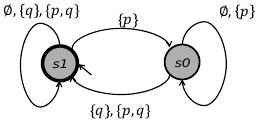
\includegraphics{pics/automatpq}
\end{figure}

\f{Der Produktautomat}
\vspace*{5pt}

\noindent Gegeben seien zwei Büchi-Automaten $B_1=(S_1,S_{1,0},A,\Delta_1,F_1)$, $B_2=(S_2,S_{2,0},A,\Delta_2,F_2)$ als Akzeptoren zweier $\omega$ regulärer
Sprachen $L(B_1),L(B_2)$:  \\ wir definieren den \f{Produktautomaten} $B_{1\times2} =(S_{1\times2},S_{1\times2,0},A,\Delta_{1\times2},F_{1\times2})$ durch 
\begin{itemize}
 \item $S_{1\times2} := S_1\times S_2$
 \item $S_{1\times2,0} := S_{1,0}\times S_{2,0}$
 \item $\Delta_{1\times2} := \{((s_1,s_2),a,(t_1,t_2))|(s_1,a,t_1)\in \Delta_1 \wedge (s_2,a,t_2)\in \Delta_2\}$
 \item $F_{1\times2} := F_1\times F_2$
\end{itemize}
\vspace*{6pt}
\f{LTL-Model-Checking}
\vspace*{5pt}

\noindent Wir haben nun eine Möglichkeit entwickelt, mit der man (im Prinzip, schnelle Heuristiken sind nach wie vor Gegenstand der aktuellen Forschung) Model 
Checking für LTL Formeln algorithmisch durchführen kann:

\noindent Gegeben sei eine Kripke-Struktur $K=(S,\rightarrow, St,AP,L)$ und eine LTL-Formel $\Phi$ über $AP$. Entscheide, ob $[[K]] \subseteq [[\Phi]]$.
\begin{enumerate}
 \item die Kripke Struktur $K$ stammt in der Regel von einer Spezifikation des Systems in Form eines Automaten. Bei unendlichem Betrieb lässt sich diese leicht 
 durch einen Büchi-Automaten $BA(K)$ ausdrücken. 
 \item übersetze die LTL Formel $\Phi$ in einen Büchi-Automaten $BA(\neg\Phi)$ der die Sprache $[[\Phi]]$ akzeptiert.
 \item bilde den Produktautomaten $BA(L(BA(K)))\cap L(BA(\neg\Phi))$ und entscheide, ob  die Menge der akzeptierenden Läufe leer ist. 
 \item gibt es einen akzeptierenden Lauf, ist dieser ein Gegenbeispiel.
\end{enumerate}

\section*{Chapter 2.3}
\f{Baum-Zeit-Logik}

\noindent Linear-Zeit Logik ist eine Logik, die sich auf alle unendlichen Sequenzen von Belegungen mit atomaren Eigenschaften bezieht. Es gibt nur eine 
mögliche Zukunft. Man kann nicht über alternative Möglichkeiten den Entwicklung Aussagen machen. Baum-Zeit Logik erlaubt Aussagen über die Möglichkeiten eines
Systems. Prominentester Vertreter ist CTL (Computation Tree Logic).
\vspace*{5pt}

\noindent Beispiel (siehe Bild): $\Rightarrow$ lässt sich nicht in LTL adäquat beschreiben. Es gibt sowohl Folgen, in denen $p$ nie gilt, als auch Folgen, in denen $p$ 
irgendwann mal gilt. 

\begin{figure}[!ht]
 \centering
 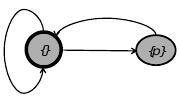
\includegraphics{pics/ctl}
\end{figure}

\f{Belegungsbaum zu einer Kripke-Struktur}:
\vspace*{4pt}

\noindent Sei $K=(S,\rightarrow,s_0,AP,L)$ eine Kripke-Struktur mit Startzustand $s_0$. Für $s\in S$ sei ein Belegungsbaum $T_K(s)$ zu $K$ mit Wurzel $s$ wie folgt
definiert: 
\vspace*{4pt}

\noindent Zu jedem $s'\in S$ mit $s\rightarrow s'$ gibt es genau einen zu $T_K(s')$ isomorphen Unterbaum von $T_K(s)$. 
\vspace*{4pt}

\noindent $T_K(s)$ beschreibt quasi eine Entfaltung der Kripke-Struktur in einen unendlich tiefen Baum. 
\vspace*{5pt}

\noindent CTL-Formeln werden über Berechnungsbäume interpretiert. Sie machen bei jedem temporalen Operator eine Aussage über die Menge der möglichen 
Entwicklungen im Baum durch existenzielle oder universelle Quantifizierung.
\vspace*{5pt}

\f{Syntax von CTL}:
\vspace*{4pt}

\noindent Sei $AP$ eine Menge von atomaren Aussagen. Dann ist die Menge der CTL-Formeln über $AP$ wie folgt definiert: 
\begin{itemize}
 \item jedes $p\in AP$ ist eine CTL-Formel
 \item sind $\Phi_1$ und $\Phi_2$ Formeln, dann auch $\neg\Phi_1$, $\Phi_1 \vee\Phi_2$, $\f{EX}\Phi_1$, $\f{EG}\Phi_1$,$\Phi_1\f{EU}\Phi_2$
 \item nichts sonst ist eine CTL-Formel
\end{itemize}
\f{EX} \dots exists next, \f{EG} \dots exists globally und \f{EU} \dots exists until sind temporale Operatoren.

\noindent Alle anderen Operatoren kann man durch Formeln über diese ausdrücken. 
\vspace*{5pt}

\f{Nützliche Abkürzungen für CTL-Formeln}:
\begin{itemize}
 \item $\Phi_1\wedge\Phi_2 \equiv \neg(\neg\Phi_1\vee\neg\Phi_2)$
 \item $true \equiv a\vee\neg a$
 \item $\f{EF}\Phi \equiv true\f{EU}\Phi$
 \item $\f{AX}\Phi \equiv \neg\f{EX}\neg\Phi$
 \item $\f{AF}\Phi \equiv \neg\f{EG}\neg\Phi$
 \item $\Phi_1\f{AU}\Phi_2 \equiv \f{AF}\Phi_2 \wedge (\Phi_1\f{AW}\Phi_2)$
 \item $\Phi_1 \rightarrow \Phi_2 \equiv \neg\Phi_1\vee\Phi_2$
 \item $false \equiv \neg true$
 \item $\Phi_1\f{EW}\Phi_2 \equiv (\Phi_1\f{EU}\Phi_2)\vee\f{EG}\Phi_1$
 \item $\f{AG}\Phi \equiv \neg\f{EF}\neg\Phi$
 \item $\Phi_1\f{AW}\Phi_2 \equiv \neg(\neg\Phi_2\f{EU}\neg(\Phi_1\vee\Phi_2))$
\end{itemize}
\f{A} \dots all (für alle Pfade), \f{F} \dots future, \f{W} \dots weak until
\vspace*{5pt}

\f{Beispiele: siehe Übungsblätter}

\end{chapter}
